\section*{Appendix}

\paragraph{Definition: Fourierserie och Fouriertransform. \\}
Eulers formel ger att $e^{i \cdot x} = cos(x) + i \cdot sin(x)$ Men går det att uttrycka en funktion som en oändlig summa
med sinus och cosinusvågor?\\
Mer matematisk blir frågan om kan man skriva en funktion $f(t)$ som 
\[
	f(t) = \sum_{n = - \infty}^\infty C_n \cdot e^{i \cdot n \cdot t}
\]
Detta går om $f(t)$ är periodisk med perioden $2 \pi$. Om så är fallet gäller:
\begin{align*}
	&f(t) = \sum_{n = - \infty}^\infty C_n \cdot e^{i \cdot n \cdot t} \\
	&f(t) \cdot e^{-imt} = \sum_{n = - \infty}^\infty C_n(e^{i(n - m) \cdot t}) \\
	&\int_{-\pi}^\pi f(t) \cdot e^{-imt}\; dt= \int_{-\pi}^\pi \sum_{n = - \infty}^\infty C_n \cdot e^{i(n - m) \cdot t}\; dt=
	\sum_{n = - \infty}^\infty C_n \cdot \int_{-\pi}^\pi e^{i (n - m) \cdot t}\; dt\\
\end{align*}
Integralen på höger sida $= 0 $ om $n \ne m$ och $= 2\pi $ om $n = m$
\[
	\int_{-\pi}^\pi f(t) \cdot e^{-i \cdot m \cdot t}\; dt 
		= C_n \cdot 3\pi = C_m \cdot 2\pi \Leftrightarrow C_m 
		= \frac 1 {2\pi} \cdot \int_{-\pi}^\pi f(t) \cdot e^{i \cdot m \cdot t}\; dt
\]
Mer generellt så gäller att om $f(t)$ har en Period $L$ så är:
\begin{align*}
	f(t) &= \sum_{n = - \infty}^\infty C_n \cdot e^{i \cdot n \cdot 2\pi \cdot \frac t L} \\ %att \fraca eller att inte \fraca
	\text{där } C_n &= \frac 1 L \int_{- L / 2}^{L / 2} f(t) \cdot e^{- \frac {i \cdot n \cdot 2\pi} {L}} 
\end{align*} %det här måste kollas till. Gränserna på integralen och aligningen på texten samt ekvationerna

där $C_n$ kallas för den n:te Fourierkoefficienten till $f(t)$. \\
Fouriertransformen av en funktion f(t) definieras som:
\[
	\mathcal{F}(u) = \frac 1 {2\pi} \cdot
	\int_{-\infty}^\infty f(t) \cdot e^{- i \cdot u \cdot t} \; dt
\]
\paragraph{Sats 1:} 
$\sum\limits_{n \in \mathbb{Z}} f(n) = \sum\limits_{n \in \mathbb{Z}} \hat{f}(m)$ där $\hat{f}(m)$ är Fouriertransformen till $f(n)$.
\\
{\bf Bevis:} \\
Vi börjar med att definiera $g(x)$ som $\sum\limits_{n \in \mathbb{Z}} f(x + n)$ eftersom $g(x)$ är periodisk med perioden $1$
kan vi skriva ett uttryck för dess Fourierkoefficienter.
\begin{align*}
	\hat{g_k} &= \int_0^1 \sum_{n \in \mathbb{Z}} f(x + n) \cdot e^{-ikx}\; dx \\
			  &= \sum_{n \in \mathbb{Z}} \int_0^1 f(x + n) \cdot e^{-ikx}\; dx \\
			  &= \sum_{n \in \mathbb{Z}} \int_n^{n + 1} f(x) \cdot e^{-ikx}\; dx \\
			  &= ... \int_{-1}^0 f(x) \cdot e^{-ikx}\; dx + \int_0^1 f(x) - e^{-ikx}\; dx + \int_1^2 f(x) \cdot e^{-ikx}\; dx ... \\
			  &= \int_{- \infty}^\infty f(x) \cdot e^{-ikx}\; dx = \hat{f}(x)
\end{align*}
Som är fouriertransformen av $f(x)$.
\[
	g(x) = \sum_{n \in \mathbb{Z}} f(x + n) = \sum_{k \in \mathbb{Z}} \hat{f}(k) \cdot e^{ikx}%ska det vara -ikx?
\]
som är fourierserien till $g(x)$. Om vi nu väljer $x = 0$ får vi:
\[
	\sum_{n \in \mathbb{Z}} f(n) = \sum_{k \in \mathbb{Z}} \hat{f}(k) \cdot e^0 = \sum_{k \in \mathbb{Z}} \hat{f}(k)
\]
$\hfill \qed$

\paragraph{Sats 2:}
Om $f(z) = u(x, y) + iv(x, y)$ är differentierbar i punkten $z_0 = x_0 + iy_0$ måste:
\newcommand{\du}[2] {
	\frac {d #1} {d #2} 
}
\[
	\du u x = \du v y \text{ och }
	\du u y = -\du v x
\]
{\bf Bevis:}
\\
Vi utgår från derivatans definition:
$$f'(z_0) = \lim_{\Delta z \to 0} \frac {f(z_0 + \Delta z) - f(z_0)} {\Delta z} $$
$\Delta z = \Delta x + i \Delta y$ får gå mot $0$ från alla riktningar i det komplexa planet.
Om $\Delta z \to 0$ horisontellt är $\Delta z = \Delta x$ och vi får då:
\newcommand{\xtz} {
	\Delta x \to 0
}
\newcommand{\bracketDelta}[4] {
	\lim_{\Delta #1 \to 0} \left [
		\frac {
			#2(x_0, #3) - #2(x_0, y_0)
		} {
			#4
		}
	\right ]
}

\newcommand{\uberBracket}[6] {
	\begin{align*}
		&= \bracketDelta #2 u #3 #4 + i \bracketDelta #2 v #3 #4 \\
		&= #5 \frac {d u} {d #2} (#2_0, #6_0) + i \frac {dv} {d #2} (x_0, y_0) = f'(z_0)
	\end{align*}
}

\uberBracket{
	f'(z_0) &= \lim_{\xtz} \frac {
		u(x_0 + \Delta x, y) + iv(x_0 + \Delta x, y) - u(x_0, y_0) - iv(x_0, y_0)
		} {
			\Delta x
		} \\
} {x} {+ \Delta x,y} {\Delta x} {} {y}

\begin{align*}
	f'(z_0) &=  \lim_{\xtz} \frac {
		u(x_0 + \Delta x, y) + iv(x_0 + \Delta x, y) - u(x_0, y_0) - iv(x_0, y_0)
	} {
		\Delta x
	} \\
	&= \bracketDelta x u {+ \Delta x,y} {\Delta x} 
	+ i \bracketDelta x v {+ \Delta x,y} {\Delta x} \\
	&= \frac {d u} {d x} (x_0, y_0) + i \frac {d v} {d x} (x_0, y_0) = f'(z_0)
\end{align*}
Om $\Delta z \to 0$ vertikalt är $\Delta z = i \Delta y$ och $vi$ får då:
\begin{align*}
	f'(z_0)
	&= \bracketDelta y u {y_0 + \Delta y} {i \Delta y}
	+ i \bracketDelta y v {y + y_0 + \Delta y} {i\Delta y} \\
	&= - i \frac {d u} {d y} (x_0, y_0) + \frac {d v} {d y} (x_0, y_0) = f'(z_0)
\end{align*}
Om vi sätter real-delarna lika med varandra och imaginärdelarna lika med varandra får vi:
$$\frac {d u} {d x} = \frac {d v} {d y}, \frac {d u} {d y} = -
	\frac {d v} {d x}$$
\hfill \qed

\paragraph{Definition 1: Klass $C_1$}
Låt $f$ vara definierad i en mängd $D$. Vi säger att $f$ är av klass $C_1$ om $f$ är partiellt deriverbar och
alla de partiella derivatorna är kontinuerliga i $D$.\\
\\
\paragraph{Sats 3:} För två funktioner av klass $C_1, P(x, y)$ och $Q(x, y)$ gäller det att:
$$\int_{\partial D} P\; dx + Q \; dy = \iint_D \left ( \frac {d Q} {d x} - \frac {d P} {d y}
	\right ) \; dx \; dy$$\\
$$\text{Där $D$ är ett kompakt område och $\partial D$ är randen till $D$.}$$
\\
{\bf Bevis:} \\
Beviset genomförs under förutsättningen att $D$ med räta linjer, parallella med y-axeln, kan delas upp i ett 
ändligt antal områden av typen:
$$E \{ (x, y): \psi(x) \le y \le \varphi(x), a \le x \le b \}$$
Och att det finns en motsvarande uppdelning för x-axeln
%bild!!!!
\begin{center}
	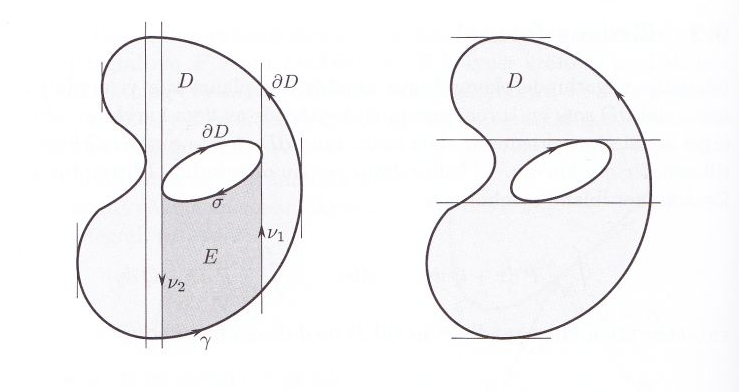
\includegraphics[scale=0.5]{linus_0001.jpg}
	{\it Figur 1}
\end{center}
Inledningsvis visas det att:
$$\int_{\partial E} P \; dx = \iint_E - \frac {dP} {dy} \; dx \; dy$$
$$\iint_E - \frac {dP} {dy} \; dx \; dy = \int^b_{x=a} \left [ -P (x, y) \right ]^{x = \varphi(x)}_{x= \psi(x)} \; dx$$
\begin{align}
	\int_a^bP(x, \psi(x)) \; dx - \int_b^aP(x, \varphi(x)) \; dx
\end{align}
Kurvan $\gamma$ i figuren kan framställas med $x$ som parameter:
$$\gamma = (x, \psi(x)), a\le x \le b.$$
Den första integralen i $(1)$ kan därför skrivas som 
$$\int_{\gamma} P \; dx + 0 \; dy = \int_{\gamma} P \; dx. \; (2)$$
På samma sätt får vi för den andra termen att:
$$- \int_a^b P(x, \varphi(x)) \; dx = \int_{\sigma} P \; dx \; (3)$$ %vad är det här för en variabel?
då kurvintegralen av de (eventuella) randstyckena $v_1$ och $v_2$ är noll innebär detta att
addition av $(2)$ och $(3)$ ger $\int_{\partial E} P \; dx$, vilket
innebär att:
$$\int_{\partial E} P \; dx = \iint_E - \frac {dP} {dy} \; dx dy.$$
genom att addera ihop det här resultatet för alla uppkommande områden av $E$ ger detta:
$$\int_{\partial D} P \; dx = \iint_D - \frac {dP} {dy} \; dx dy.$$
Om vi gör på samma sätt med en uppdelning av $D$ med linjer parallella med X-axeln får vi på liknande sätt att:
$$\int_{\partial D} Q \; dy = \iint_D \frac {dQ} {dx} \; dy dx.$$ 
genom att addera uttrycken följer nu att:
$$\iint_D \left ( \frac {dQ} {dx} - \frac {dP} {dy} \right ) \; dx dy = \int_{\partial D} P \; dx + Q \; dy.$$
\hfill \qed
\paragraph{Definition 2:} En funktion $f$ är analytisk i ett område $D$ om den har en derivata i alla punkter i $D$.\\
\\
\paragraph{Sats 4:} Om $\Gamma$ är en sluten kurva i det komplexa talplanet och $f(z)$ är analytisk i området som innesluts av $\Gamma$ så är:
$$\int_{\Gamma} f(z) \; dz = 0.$$
\\
{\bf Bevis:}\\
Med den vanliga notationen:\\
$f(z) = u(x, y) + iv(x, y)$ får vi:
$$\int_{\Gamma} f(z) \; dz = \int_a^b f(z(t)) \frac {dz(t)} {dt} \; dt = \int_a^b [a(x(t), y(t)) + iv(x(t), y(t)) ]
\left ( \frac {dx} {dt} + i \frac {dy} {dt} \right ) \; dt$$

$$= \int_a^b \left [a(x(t), y(t)) \frac {dx} {dt} - v(x(t), y(t)) \frac {dy} {dt} \right ] \; dt + i \int_a^b \left [v(x(t), y(t)) \frac {dx} {dt} + 
u(x(t), y (t)) \frac {dy} {dt} \right ] \; dt$$

$$\int_{\Gamma} f(z) \; dz = \int_\Gamma (u \; dx - v \; dy) + i \int_\Gamma v \; dx + u \; dy$$
Sats 3 ger nu:
$$\int_{\Gamma} f(z) \; dz = \iint_{D^\prime} \left ( - \frac {dv} {dx} - \frac {du} {dy} \right ) \; dxdy +
i \iint_{D^\prime} \left ( \frac {du} {dx} - \frac {dv} {dy} \right ) \; dxdy$$

där $D'$ är området som innesluts av $\Gamma$. Men ekvationerna från Sats 2 ger nu att
dubbelintegralerna är $0$. vilket ger:
$$\int_\Gamma f(z) \; dz = 0$$
\hfill \qed

\paragraph{Sats 5:} $f(z_0) = \frac 1 {2\pi i} \cdot \int_\Gamma \frac {f(z)} {z - z_0} \; dz$ \\
\\
{\bf Bevis:}\\
$\frac {f(z)} {z - z_0}$ är analytisk överallt i området som innesluts av $\Gamma$ förutom i punkten
$z = z_0$. Vi kan därför deformera $\Gamma$ till en cirkel $C_r$ med radien $r$ och 
som är centrerad kring $z_0$.

\[ \int_\Gamma \frac {f(z)} {z - z_0} \; dz = \int_{C_r} \frac {f(z)} {z - z_0} \; dz. \]

\[ \int_{C_r} \frac {f(z)} {z - z_0} \; dz = \int_{C_r} \frac {f(z) - f(z_0) + f(z_0)} {z - z_0} \; dz =
	\int_{C_r} \frac {f(z_0)} {z - z_0} \; dz + \int_{C_r} \frac {f(z) - f(z_0)} {z - z_0} \; dz \;(1) \]

substitutionen 
\begin{align*}
	z  &= r \cdot e^{iv} + z_0 \\
	dz &= r \cdot i \cdot e^{iv} \; dv
\end{align*}
ger i den vänstra integralen:
\[ \int_{C_r} \frac {f(z_0)} {z - z_0} \; dz = \int_0^{2\pi} \frac {f(z_0) \cdot r \cdot i \cdot e^{iv} } { r \cdot e^{iv}} \; dv =
	\left [f(z_0) \cdot iv \right ]_0^{2\pi} = f(z_0) \cdot 2 \pi i. \]

den högra integralen i $(1) \rightarrow 0$ då radien av cirkeln $\rightarrow 0$.
Detta visas genom att sätta $M_r := \operatorname{max} [|f(z) - f(z_0)|; z \text{ på } C_r]$
Detta innebär att

\[
	\left | \frac {f(z) - f(z_0)} {z - z_0} \right | = \frac {|f(z) - f(z_0)|} {r} \leq \frac {M_r} {r}
\]

\[
	\left | \int_{C_r} \frac {f(z) - f(z_0)} {z - z_0} \; dz \right | \leq \frac {M_r} {r} l(C_r)
\]
där $l(C_r)$ är längden av kurvan $C_r$.

\[
\frac {M_r} {r} \cdot l(C_r) = \frac {M_r} {r} \cdot 2r\pi = M_r \cdot 2 \pi
\]
men då $f$ är kontinuerlig i punkten $z_0$ går $M_r \rightarrow 0$ då $r \rightarrow 0$.
Alltså är $\int_{C_r} \frac {f(z) - f(z_0)} {z - z_0} \; dz = 0.$ Vilket innebär att $(1) = 2\pi i \cdot f(z_0) + 0$
division med $2\pi i$ ger:
\[
	f(z_0) = \frac {1} {2 \pi i} \cdot \int_{\Gamma} \frac {f(z)} {z - z_0} \; dz.
\]
\hfill \qed
\\

\paragraph{Sats 6:}
\[
	f^{(n)}(z_0) = \frac {1} {2 \pi i} \cdot \int_{\Gamma} \frac {f(z)} {(z - z_0)^{(n + 1)}} \; dz \cdot n!
\]
\\
{\bf Bevis:}\\
Detta inses genom att derivera uttrycket med avseende på $z_0$.
\begin{align*}
	f(z_0) &= \frac {1} {2 \pi i} \cdot \int_{\Gamma} \frac {f(z)} {(z - z_0)} \; dz = \frac {1} {2 \pi i} \cdot \int_{\Gamma}
		f(z) \cdot (z - z_0)^{-1} \; dz \\
	f'(z_0) &= \frac {1} {2 \pi i} \cdot -1 \cdot -1 \cdot \int_{\Gamma} f(z) \cdot (z - z_0)^{-2} \; dz \\
	f''(z_0) &= \frac {1} {2 \pi i} \cdot -1 \cdot -2 \cdot \int_{\Gamma} f(z) \cdot (z - z_0)^{-3} \; dz \\
	f'''(z_0) &= \frac {1} {2 \pi i} \cdot 2 \cdot -1 \cdot -3 \cdot \int_{\Gamma} f(z) \cdot (z - z_0)^{-4} \; dz \\
	\vdots \\
	f^{(n)}(z_0) &= \frac {1} {2 \pi i} \cdot n! \cdot \int_\Gamma f(z) \cdot (z \ z_0)^{-(n + 1)} \; dz
\end{align*} %jag fattade inget av Sats 5, jag tror att det är fel
\hfill \qed
\\
\paragraph{Sats 7:}
\[
	f(z) = \sum_{j = - \infty}^\infty a_j (z - z_0)^j. \text{ med } a_j = \frac {1} {2 \pi i} \cdot \ointctrclockwise
		\frac {f(\zeta)} {(\zeta - z_0)^{j + 1}} \; d\zeta
\]
Detta kallas för en Laurent-serie\\
\\
{\bf Bevis:}\\
Låt $\Gamma$ vara en sluten kurva runt $z$.
Låt därefter $\Gamma$ se ut som en ``donut'' med en ``bit'' borta.
%biiild
\begin{center}
	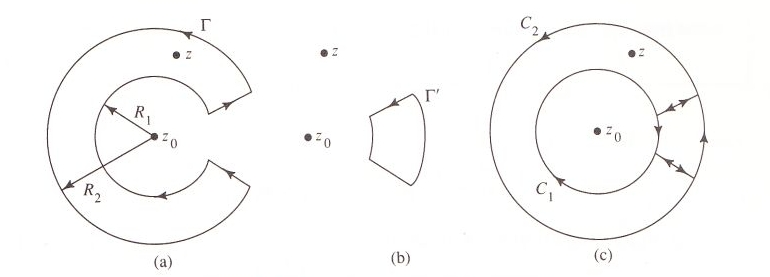
\includegraphics[scale=0.5]{aoeu.jpg}
	{\it Figur 2}
\end{center}
Låt $\Gamma'$ vara den ``borttagna biten''. då $f(z)$ är analytisk i hela området som innesluts av $\Gamma'$ ger Sats 3 att.
\[
	\frac {1} {2 \pi i} \int_{\Gamma'} \frac {f(\zeta)} {\zeta - z} \; d\zeta = 0
\]
därmed följer att vi kan ``sätta tillbaka biten''. Då integralen var $= 0$ följer att:
\[
	f(z) = \frac {1} {2 \pi i} \cdot \int_{\Gamma + \Gamma'} \frac {f(\zeta)} {\zeta - z} \; dz
\]
då integralerna längs linjesegmenten tar ut varandra följer det att:
\[
	f(z) = \frac {1} {2 \pi i} \left ( \varointclockwise_{C_1} \frac {f(\zeta)} {\zeta - z} \; d\zeta + 
		\ointctrclockwise_{C_2} \frac {f(\zeta)} {\zeta - z} \; d\zeta \right ) \quad (1)
\]
\[
	f(z) = \sum_{k = 0}^\infty \frac {f^{(n)}(z_0)} {n!} (z - z_0)^n \quad \text{ (taylorpolynom) }
\]

Sats 6 ger nu:
\[
	f(z) = \sum_{n = 0}^\infty a_n (z - z_0)^n = \frac {1} {2 \pi i} \cdot \ointctrclockwise_{C_2} \frac 
		{f(\zeta)} {\zeta - z} \; d\zeta
\]
Om man nu fokuserar på integralen runt $C_1$ i $(1)$ så ser man att då $z$ ligger utanför $C_1$ 
måste vi integrera kring en annan punkt.
\[
	\frac {1} {\zeta - z} = \frac {1} {(\zeta - z) - (z - z_0)} = - \frac {1} {(z - z_0)}
		\left (
			\frac {1} {1 - \frac {(\zeta - z_0)} {(z - z_0)}}
		\right )
\]
taylorpolynomet till den högra faktorn ger nu:
\[
	- \frac {1} {(z - z_0)} \cdot \sum_{k = 0}^\infty
		\left (
			\frac {(\zeta - z_0)} {(z - z_0)}
		\right )^k
\]
insättning i integralen ger nu:
\[ %wuuuut
	- \frac {1} {2 \pi i} \varointclockwise_{C_1} f(\zeta) \cdot \sum_{k = 1}^\infty \frac {(\zeta - z_0)^{k - 1}} {(z - z_0)^k} \; d\zeta
	= \sum_{k = 1}^\infty -\frac{1} {2 \pi i} \cdot \varointclockwise_{C_1} \frac {f(\zeta)} {(\zeta - z_0)^{-k + 1}} \; d\zeta \cdot
			(z - z_0)^{-k} = \sum_{k = 1}^\infty a_{-k} (z - z_0)^{-k}
\] %överväg radbrytning
Där $a_{-k} = -\frac{1} {2 \pi i} \cdot \varointclockwise_{C_1} \frac {f(\zeta)} {(\zeta - z_0)^{-k + 1}} \; d\zeta$.
%\[
%	= \sum_{k = 1}^\infty a_{-k} (z - z_0)^{-k}
%\]
Ekvation $(1)$ blir nu:
\[
	\sum_{n = 0}^\infty a_n(z - z_0)^n + \sum_{k = 1}^\infty a_{-k}(z - z_0)^{-k}
\]
\hfill \qed

\paragraph{Sats 8:}
Om $f$ har en singularitet i punkten $z_0$ så är linjeintegralen runt singulariteten $= 2 \pi i \cdot a_{-1}$.\\
\\
{\bf Bevis:}\\
Sats 7 ger att $f(z) = \sum\limits_{j = - \infty}^\infty a_j (z - z_0)^j$
\[
	\ointctrclockwise_{C_r} f(z) \; dz = \sum_{j = - \infty}^\infty a_j \cdot \ointctrclockwise_{C_r} (z - z_0)^j \; dz
\]
\begin{align*}
	z &= e^{iv} + z_0 \\
	dz &= ie^{iv} dv \qquad \text{ för } j \neq - 1
\end{align*}
\[
	\ointctrclockwise_{C_r} (z - z_0)^j \; dz = \int_0^{2 \pi} ie^{ir(j + 1)} \; dv =
	\left [
		i \frac {e^{iv(i + 1)}} {i (j + 1)}
	\right ]_0^{2 \pi}
	= 0
\]
\[
	\text{för } j = -1 \text{ gäller: } \int_0^{2\pi} ie^{iv(-1 + 1)} \; dv = 
	\left [
		i \cdot v
	\right ]_0^{2\pi}
	= 2 \pi i
\]
för alla $j \neq -1$ blir integralen $ = 0$ och för $j = -1$ blir integralen lika med $2 \pi i a_{- 1}$.
Alltså:
\[
	\ointctrclockwise_{C_r} f(z) \; dz = 2 \pi i \cdot a_{-1}
\]
där termen $a_{-1}$ kallas för residualen \\
\hfill \qed

\paragraph{Sats 9:} $a_{-1} = \lim_{z \to z_0} f(z) \cdot (z - z_0)$\\
\\
{\bf Bevis:}\\
Om $f(z)$ har en ``borttagbar'' singularitet i Punkten $z = z_0 \qquad \left ( \frac {1} {z - z_0} \right )$ blir 
alla koefficienter till $f(z)$'s Laurentserie för $j < -1 = 0$. Detta på grund av att integralen i $a_k$ för $k < -1$
inte innesluter en singularitet, och integralen  är därmed, enligt Sats 3, lika med $0$.
Men om $f(z)$ har en singularitet i punkten $z = z_0$ gäller:
\begin{align*}
	&f(z) = \frac {a - 1} {z - z_0} + a_0 + a_1(z - z_0) + a_2(z - z_0)^2 \ldots \\
	&f(z) (z - z_0) = a_{-1} + (z - z_0)(a_0 + a_1 (z - z_0) \ldots ) \\
	\lim_{z \to z_0} &f(z)(z - z_0) = a_{- 1} + (0)(a_0 + a_1(z - z_0) \ldots ) = a_{-1}
\end{align*}
\hfill \qed
\\
\paragraph{Sats 10:} %kanske ska ändra till "implicerar"
Om $A_n = \sum\limits_{i = 0}^n a_1, \quad \text{ då är } \sum\limits_{i = 0}^n a_i \cdot b_i = 
		\sum\limits_{i = 0}^{n - 1} A_i (b_i - b_{i + 1}) + A_n \cdot b_n$\\
{\bf Bevis:}\\
\\
\[ a_k = A_k - A_{k - 1} \]
\[
	\sum_{k = 0}^n a_k \cdot b_k =  \sum_{k = 0}^n (A_k - A_{k - 1}) \cdot b_k = \sum_{i = 0}^n A_k \cdot b_k - 
		\sum_{k = 0}^n A_{k - 1} \cdot b_k
\]
i den andra summan substitueras $k$ mot $i + 1$
\[
	\sum_{k = 0}^n A_{k - 1} \cdot b_k = \sum_{i = 0}^{n - 1} A_i \cdot b_{i + 1} = \sum_{k = 0}^{n - 1} A_k \cdot b_{k + 1}
\]
vi har nu
\[
	\sum_{k = 0}^n a_k \cdot b_k = \sum_{k = 0}^n A_k \cdot b_k - \sum_{k = 0}^{n - 1} A_k \cdot b_{k + 1} =
		\sum_{k = 0}^{n - 1} A_k (b_k - b_{k + 1}) + A_n \cdot b_n
\]
\\
\paragraph{Sats 11:} $(n^{-s} - (n + 1)^{-s}) = s \cdot \int\limits_n^{n + 1} x^{-s - 1} \; dx$\\
{\bf Bevis:}\\
\[
	s \cdot \int_n^{n + 1} x^{-s - 1} \; dx = - [ x^{-s} ]_n^{n + 1} = - ((n + 1)^{-s} - n^{-s})
		= n^{-s} -(n + 1)^{-s}
\]
\hfill \qed
\\
\paragraph{Definition 3:} $\floor{x} = \text{ heltalsdelen av } x$\\
\\
exempel:\\
$\floor{\pi} = 3, \quad \floor{e} = 2, \quad \floor{38.5} = 38$\\
\\
\paragraph{Definition 4:} $\fpart{x} = x - \floor{x}$\\
\\
exempel:\\
$\fpart{\pi} = 0.14159265358979 \ldots, \quad \fpart{e} = 0.72182818284590 \ldots, \fpart{38.5} = 0.5$\\
\\
\paragraph{Sats 12:} $\frac {s} {s - 1} - s \cdot \int\limits_1^\infty \floor{x} x^{-s - 1} \; dx +
		s \cdot \int\limits_1^\infty \fpart{x} x^{-s - 1} \; dx$ \\
{\bf Bevis:}\\
\[
	s \cdot \int_1^\infty x^{-s - 1} (\floor{x} + \fpart{x}) \; dx = s \cdot \int_1^\infty x^{-s} \; dx
\]
\[
	= s \cdot \left [
		\frac {x^{-s + 1}} {-s + 1}
	\right ]_1^\infty =
	\frac {1^{1 - s}} {1 - s} \cdot s = \frac {s} {1 - s}
\]
\hfill \qed
\\
\paragraph{Sats 13:} $\zeta(s) = \frac {s} {s - 1} - s \int\limits_1^\infty \fpart{x} x^{-s - 1} \; dx$\\
\\
{\bf Bevis:}\\
\[
	\zeta(s) = \sum_{n \leq n} \frac {1} {n^{-s}}
\]
Sats 10 ger:
\[
	\sum_{n \leq 1} \frac {1} {n^{-s}} = \sum_{n \leq 1} n \cdot (n^{-s} - (n + 1)^{-s})
\]
Sats 11 ger nu att:
\[
	s \sum_{n \leq 1} n (n^{-s} - (n + 1)^{-s}) = s \sum_{n \leq 1} \int_n^{n + 1} \floor{x} x^{-s -1} \; dx =
		s \int_1^\infty \floor{x} x^{-s - 1} \; dx
\]
Sats 12 ger slutligen att:
\[
	\int_1^\infty \floor{x} x^{-s - 1} \; dx = \frac {s} {s - 1} - s \int_1^\infty \fpart{x} x^{-s - 1} \; dx = \zeta(s)
\]
\hfill \qed
\\
\paragraph{Sats 14:} $\zeta(s)$ har en singularitet i $s = 1$ med residualen $1$.\\
\\
{\bf Bevis:}\\
Sats 9 visar att residualen $= \lim_{z - z_0} f(z)(z - z_0)$
\[
	\zeta(s) - (s - 1) = \left (
		\frac {s} {s - 1} - s \cdot \int_1^\infty \fpart{x} x^{-s - 1} \; dx 
		\right )
	(s - 1)
\]
\[
	\lim_{s \to 1} \zeta(s)(s - 1) = \lim_{s \to 1} s - s (s - 1) \cdot \int_1^\infty \fpart{x} x^{-s - 1} \; dx =
		1 - 0 = 1
\]
\hfill \qed
\end{document}


